\documentclass[../mech.tex]{subfiles}
\graphicspath{{\subfix{../figures/}}}
\begin{document}
\chapter{Oscillations}
\section{Defining Simple Harmonic Motion (SHM)}
Simple harmonic motion (SHM) is a special case of periodic motion.

SHM results when the magnitude of the restoring force exerted on an object is proportional to that object's displacement from its equilibrium position.

A restoring force is a force that is exerted in a direction opposite to the object's displacement from an equilibrium position.
\begin{itemize}
    \item An equilibrium position is a location at which the net force exerted on an object or system is zero.
\end{itemize}

\begin{example}
    A block of mass $m$ is attached to a spring, with force constant $k$, on a horizontal surface. The block is pulled to a position of $x$ and allowed to oscillate back and forth.
    The coefficient of kinetic friction between the block and the table is $\mu$. Derive an expression for the acceleration of the block and write the differential equation, but don't solve, that can be used to determine the position 
    function of the block with respect to time.

    Start with $\sum F_x = ma_x$.

    From this we get $F_{sp}-f_k = ma_x \implies -kx -\mu mg = ma_x$. Solving for $a_x$ gives $a_x = -\frac{kx}{m}-\mu g$.

    Substitute $\frac{\dd^2 x}{\dd t^2}$ for $a_x$ to get the differential equation.
\end{example}

\ex \begin{center}
    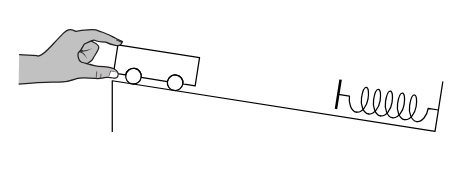
\includegraphics[width=0.5\textwidth]{7.1.PNG}
\end{center}
A cart is initially at rest near the top of a straight ramp, as shown in the figure. A spring is attached to a wall near the bottom of the ramp and is parallel to the ramp surface. The cart is released from rest, rolls down the ramp, compresses the spring, 
reverses direction, and is then launched back up the ramp by the spring. The cart returns to its initial position, and the motion repeats. Although the cart's motion is periodic, it is not simple harmonic motion. Why does the cart not undergo simple harmonic motion?

\pagebreak
\ex \begin{center}
    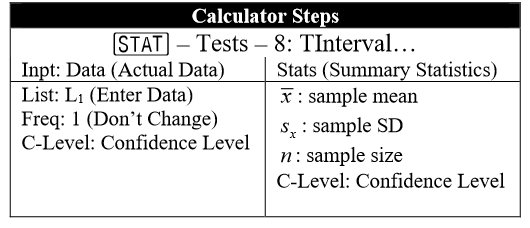
\includegraphics[width=0.5\textwidth]{7.1.2.PNG}
\end{center}
A small ball is initially at rest at the top of a smooth curved hill. The hill's surface is in the shape of a parabola. If the ball is rolled down the hill, is the $x$-component of its motion an example of simple harmonic motion? Support your claim.

\section{Frequency and Period of SHM}
The period of SHM is related to the angular frequency, $\omega$, of the object's motion by the following equation:
\[ \omega = \frac{2\pi}{T} \qquad \omega = 2\pi f \]
The period of the object-ideal spring oscillator is given by the equation:
\[ T_{sp}=2\pi \sqrt{\frac{m}{k}} \]
The period of a simple pendulum displaced by a small angle is given by the equation:
\[ T_{p}=2\pi \sqrt{\frac{l}{g}} \]

\begin{example}
    A $2.0$ m long pendulum is pulled back and allowed to swing freely on Earth. What is the frequency of the pendulum? How does the frequency of the pendulum compare to that on the Moon ($g=1.67$ m/s$^2$)?

    Plug this in to the formula to get $T_E=2.84$ s, and the frequency is $\frac{1}{2.84} = 0.352$ Hz.

    Plug into the same formula for the moon, and you get $0.445$ Hz for the frequency.
\end{example}

\ex A metal sphere is hung vertically from the bottom of a spring, and the top end of the spring is attached to the ceiling inside a car. When the car is stationary, the frequency of oscillation for the sphere-spring system is $f_0$. How does the oscillation frequency change, if at all, when the car 
starts moving forward along a horizontal road with a constant acceleration? Assume the frequency is measured by an observer at rest with respect to the road in both situations.

\pagebreak
\ex \begin{center}
    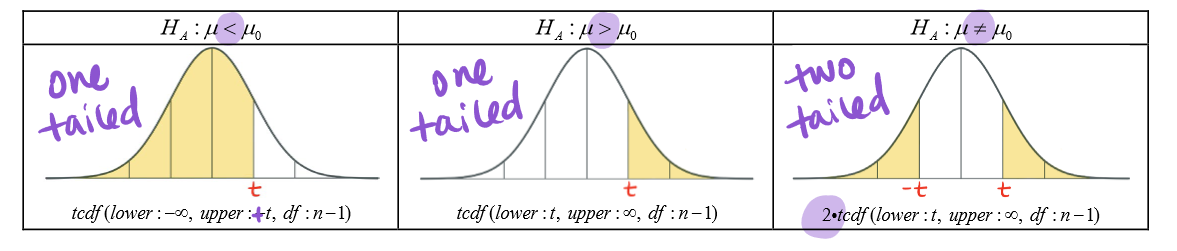
\includegraphics[width=0.5\textwidth]{7.2.1.PNG}
\end{center}
A small ball is hung from a string of length $3L_0$, as shown in the figures. There is a small peg just to the left of the string at a distance $L_0$ above the center of the ball. The ball is displaced to the left and released from rest, as shown in the middle figure, and moves 
as a pendulum of length $L_0$ until the string is vertical and loses contact with the peg. The ball then continues moving to the right as a pendulum of length $3L_0$, as shown in the right-hand figure, until the string becomes vertical and again contacts the peg. The ball continues moving to the left, 
again as a pendulum of length $L_0$, until it returns to its initial release potision and completes one oscillation, and then the motion is repeated. What is the period of a complete oscillation for the ball?

\section{Representing and Analyzing SHM}
For an object exhibiting SHM, the displacement of that object measured from its equilibrium position can be represented by the equations:
\[ x = A\cos (2\pi ft) \rightarrow x=A, t=0\]
\[ x=A\sin(2\pi ft)\rightarrow x=0, t=0\]
The position as a function of time for an object exhibiting SHM is a solution of the second order differential equation derived from the application of Newton's 2nd Law.
\[ \frac{\dd^2 x}{\dd t^2}=a=-\omega^2 x\]
Characteristics of SHM, such as velocity and acceleration can be determined by or derived from the equation:
\[ x=A\cos (\omega t + \varphi) \]
In the presence of a sinusodial external force, a system may exhibit resonance.
\begin{itemize}
    \item Resonance occurs when an external force at the natural frequency of an oscillating system and it increases the amplitude of oscillating motion.
\end{itemize}
Changing the amplitude of a system exhibiting SHM will not change its period.

Properties of SHM can be determined and analyzed using graphical representations.

\begin{example}
    A $5.0$ kg object suspended on a spring oscillates such that its position $x$ as a function of time $t$ is given by the equation $x(t)=A\cos (\omega t)$, where $A=0.80$ m and $\omega = 2.0$ s$^{-1}$. What is the 
    maximum velocity and acceleration of the object? What is the magnitude of the maximum net force on the object during the motion.

    The maximum velocity is simpliy $A\omega = (2.0)(0.8)=1.6$ m/s, likewise the acceleration is $A\omega^2 = 3.2$ m/s.

    The maximum net force is $F_{NET}=ma = 16$ N.
\end{example}

\pagebreak
\ex \begin{center}
    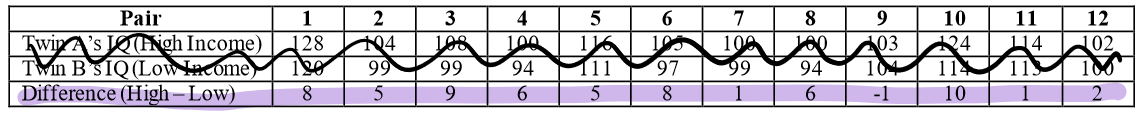
\includegraphics[width=0.5\textwidth]{7.3.1.PNG}
\end{center}
An object undergoes simple harmonic motion. The graph shows the acceleration of the object as a function of time, and at time $t_0$ the acceleration is in the positive direction as indicated. Describe the object's displacement and velocity at time $t_0$.

\ex 
\begin{center}
    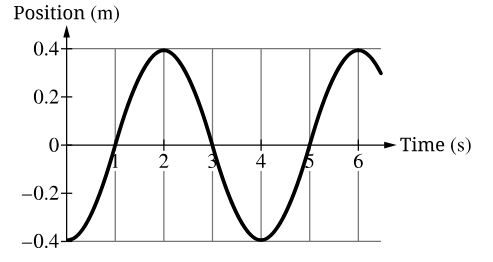
\includegraphics[width=0.5\textwidth]{7.3.2.PNG}
\end{center}
The graph shows the position $x$ as a function of time $t$ for an object in one-dimensional simple harmonic motion. Write an expression that gives the object's velocity as a function of $t$.

\section{Energy of Simple Harmonic Oscillators}
The total energy of a system exhibiting SHM is the sum of the system's kinetic and potential energies.

Conservation of energy indicates that the total energy of a system exhibiting SHM is constant.

The kinetic energy of a system exhibiting SHM is at a maximum when the system's potential energy is at a minimum, and vice versa.

Changing the amplitude of a system exhibiting SHM will change the maximum potential energy of the system and, therefore, the total energy of the system.

\begin{example}
    An object on the end of a spring with spring constant $k$ moves in simple harmonic motion with amplitude $A$ and frequency $f$. Write an expression for the kinetic energy of the object as a function of time $t$.

    Let $x=A\cos (2\pi ft)$. We know that $K_A=U_B$ and $k_A=\frac{1}{2}kA^2=\frac{1}{2}k(A\cos(2\pi ft))^2$.

    This simplifies to $K_A=\frac{1}{2}kA^2\cos^2 (2\pi ft)$.
\end{example}

\ex A block on a horizontal surface is attached to one end of a horizontal spring, and the other end of the spring is fixed in place. The block, which is free to move in the $x$-direction along the surface with negligible friction, oscillates in simple harmonic motion.
The block's mass is $2.0$ kg, and its motion has an oscillation period of $2.0$ s. When the block is $0.30$ m from the equilibrium position, it has a speed of $0.50$ m/s. What is the amplitude of the block's motion?

\pagebreak
\ex A block of mass $M_1$ is on a horizontal surface and attached to one end of a spring, while the other end of the spring is fixed in place. The block oscillates on the spring with an amplitude $A_1$ as it moves with negligible friction 
on the horizontal surface, and the block-spring system has total mechanical energy $E_1$ and maximum kinetic energy $K_1$. The block is replaced with a second block that has mass $\frac{M_1}{2}$, and the second block 
is then made to oscillate on the same spring with amplitude $2A_1$. What is the total mechanical energy and maximum kinetic energy of the second block-spring system?


\section{Simple and Physical Pendulums}
A physical pendulum is a rigid body that undergoes oscillation about a fixed axis.

For small amplitudes of motion, the period of a physical pendulum is derived from the application Newton's 2nd law of motion.

When displaced from equilibrium, the gravitational force exerted on a physical pendulum's center of mass provides a restoring torque.

The small-angle approximation and Newton's 2nd law in rotational form yield a second-order differential equation that describes SHM. 
\[ \frac{\dd^2 \theta}{\dd t^2}=-\omega^2\theta \]

A simple pendulum is a special case of physical pendulums in which the hanging object can be modeled as a point mass at a distance from the pivot point.

A torsional pendulum is a special case of SHM where the restoring torque is proportional to the angular displacement of a rotating system.

\begin{example}
    Derive an expression for the period and frequency of a torsion pendulum of torsion constant $\kappa$ and displacement $\Delta \theta$.

    We can let the torque be $-k\Delta \theta$.

    This gives us $I\alpha + k\Delta \theta = 0$.

    From this, we get $\omega^2 \theta + \frac{k\Delta \theta}{I}=0$.
\end{example}

\ex A physical pendulum is made from a uniform bar with a pivot at its top end. A second physical pendulum is made from another uniform bar of twice the length, also with a pivot at its top end. How does the small-angle oscillation period of the second pendulum compare to that of the first?
The rotational inertia about one end of a bar of mass $M$ and length $L$ is $\frac{1}{3}ML^2$.


\ex \begin{center}
    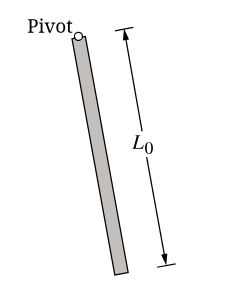
\includegraphics[width=0.2\textwidth]{7.5.1.PNG}
\end{center}
Near the surface of a distant planet, a physical pendulum made from a uniform bar of length $L_0$ exhibits small-angle oscillations about a pivot located at the top end of the bar, as shown in the figure.
The planet has $\frac{1}{40}$ the mass and $\frac{1}{5}$ the radius of Earth. The bar has mass $M_0$ and rotational inertia $I_0=\frac{1}{3}M_0L_0^2$ about the pivot axis. Write a differential equation that describes 
the pendulum's motion, where $g$ is the acceleration of gravity on Earth. The pendulum angle $\theta$ is taken relative to the vertical.

\end{document}